%----------------------------------------------------------------------------------------

\documentclass[a4paper]{article} % Uses article class in A4 format

%----------------------------------------------------------------------------------------
%	FORMATTING
%----------------------------------------------------------------------------------------

\addtolength{\hoffset}{-2.25cm}
\addtolength{\textwidth}{4.5cm}
\addtolength{\voffset}{-3.25cm}
\addtolength{\textheight}{5cm}
\setlength{\parskip}{0pt}
\setlength{\parindent}{5pt}

%----------------------------------------------------------------------------------------
%	PACKAGES AND OTHER DOCUMENT CONFIGURATIONS
%----------------------------------------------------------------------------------------

\usepackage{caption} 
\usepackage{siunitx}
\usepackage[inkscapelatex=false]{svg}
\usepackage{blindtext} % Package to generate dummy text
\usepackage[toc,page]{appendix}
\usepackage{dirtytalk}
\usepackage{bm}

\usepackage{charter} % Use the Charter font
\usepackage[utf8]{inputenc} % Use UTF-8 encoding
\usepackage{microtype} % Slightly tweak font spacing for aesthetics

\usepackage[english]{babel} % Language hyphenation and typographical rules

\usepackage{amsthm, amsmath, amssymb} % Mathematical typesetting
\usepackage{float} % Improved interface for floating objects
\usepackage[final, colorlinks = true, 
            linkcolor = black, 
            citecolor = black]{hyperref} % For hyperlinks in the PDF
\usepackage{graphicx, multicol} % Enhanced support for graphics
\usepackage{xcolor, colortbl} % Driver-independent color extensions 
\usepackage{marvosym, wasysym} % More symbols
\usepackage{rotating} % Rotation tools
\usepackage{censor} % Facilities for controlling restricted text
\usepackage{pseudocode} % Environment for specifying algorithms in a natural way
\usepackage{booktabs} % Enhances quality of tables
\usepackage{minted}
\usepackage{tikz}
\usetikzlibrary{matrix}
\usetikzlibrary{positioning}
\usetikzlibrary{calc}
\usepackage{subcaption}

\definecolor{darkgreen}{rgb}{0.12109375, 0.67578125, 0.1015625}

\newcommand{\crossnode}[2][]{
  \node[draw=none, inner sep=0pt, #1] at (#2) (cross) {};
  \draw[draw, #1] ($(cross.south west)+(-0.1,-0.1)$) -- ($(cross.north east)+(0.1,0.1)$);
  \draw[draw, #1] ($(cross.north west)+(-0.1,0.1)$) -- ($(cross.south east)+(0.1,-0.1)$);
}

\newcommand{\sddots}{\scalebox{0.75}{$\ddots$}}
\newcommand{\svdots}{\scalebox{0.75}{$\vdots$}}


\newenvironment{packed_enum}{
\begin{enumerate}
  \setlength{\itemsep}{1pt}
  \setlength{\parskip}{0pt}
  \setlength{\parsep}{0pt}
}{\end{enumerate}}

% \usepackage{tikz-qtree} % Easy tree drawing tool
% \tikzset{every tree node/.style={align=center,anchor=north},
%          level distance=2cm} % Configuration for q-trees

\usepackage[backend=biber,style=numeric,
            sorting=nyt]{biblatex} % Complete reimplementation of bibliographic facilities
\addbibresource{ecl.bib}
\usepackage{csquotes} % Context sensitive quotation facilities

\usepackage[yyyymmdd]{datetime} % Uses YEAR-MONTH-DAY format for dates
\renewcommand{\dateseparator}{-} % Sets dateseparator to '-'

\usepackage{fancyhdr} % Headers and footers
\pagestyle{fancy} % All pages have headers and footers
\fancyhead{}\renewcommand{\headrulewidth}{0pt} % Blank out the default header
\fancyfoot[L]{University of Manchester} % Custom footer text
\fancyfoot[C]{} % Custom footer text
\fancyfoot[R]{\thepage} % Custom footer text

\newcommand{\note}[1]{\marginpar{\scriptsize \textcolor{red}{#1}}} % Enables comments in red on margin


\usepackage{enumitem}
\setlist[enumerate]{itemsep=0mm}

%----------------------------------------------------------------------------------------

\begin{document}

%----------------------------------------------------------------------------------------
%	TITLE SECTION
%----------------------------------------------------------------------------------------

\title{template_assignment (UOM)} % Article title
\fancyhead[C]{}
\hrule \medskip % Upper rule
\begin{minipage}{0.295\textwidth} % Left side of title section
\raggedright
COMP36212\\ % Your lecture or course
\footnotesize % Authors text size
\hfill\\
Aaron Panaitescu, 10834225% Your name, your matriculation number`
\end{minipage}
\begin{minipage}{0.4\textwidth} % Center of title section
\centering 
\large % Title text size
Numerical Solution of the Heat Conductance Equation
\\ % Assignment title and number
\end{minipage}
\begin{minipage}{0.295\textwidth} % Right side of title section
\raggedleft
\today\\ % Date % Your email
\end{minipage}
\medskip\hrule % Lower rule
\bigskip

%----------------------------------------------------------------------------------------
%	ARTICLE CONTENTS
%----------------------------------------------------------------------------------------

\begin{multicols}{2}
[
\section{Introduction}
]
\subsection{Motivation}
Numerical solutions are approximate ~answers obtained~ through computational methods for problems that are difficult or impossible to solve analytically.
\par
This report analyses different numerical methods for solving the heat conductance equation, given by the parabolic PDE in equation \ref{eq:1}.
\begin{align} \label{eq:1}
\frac{\partial^2 T(x,t)}{\partial x^2} = \frac{1}{k}\frac{\partial T(x,t)}{\partial t}
\end{align}

\subsection{Problem statement}
This equation describes evolution in time of the temperature distribution across a one-dimensional homogeneous bar of length $L = 100\ \mathrm{ cm}$ and thermal conductivity $k = 0.875\ \mathrm{cm}^2\mathrm{s}^{-1}$. The boundary conditions are $T(x,0)=500\ ^\circ \mathrm{C}$ and $T(0,t) = T(0,L) = 0\ ^\circ \mathrm{C}$.

\begin{figure}[H]
    \centering
    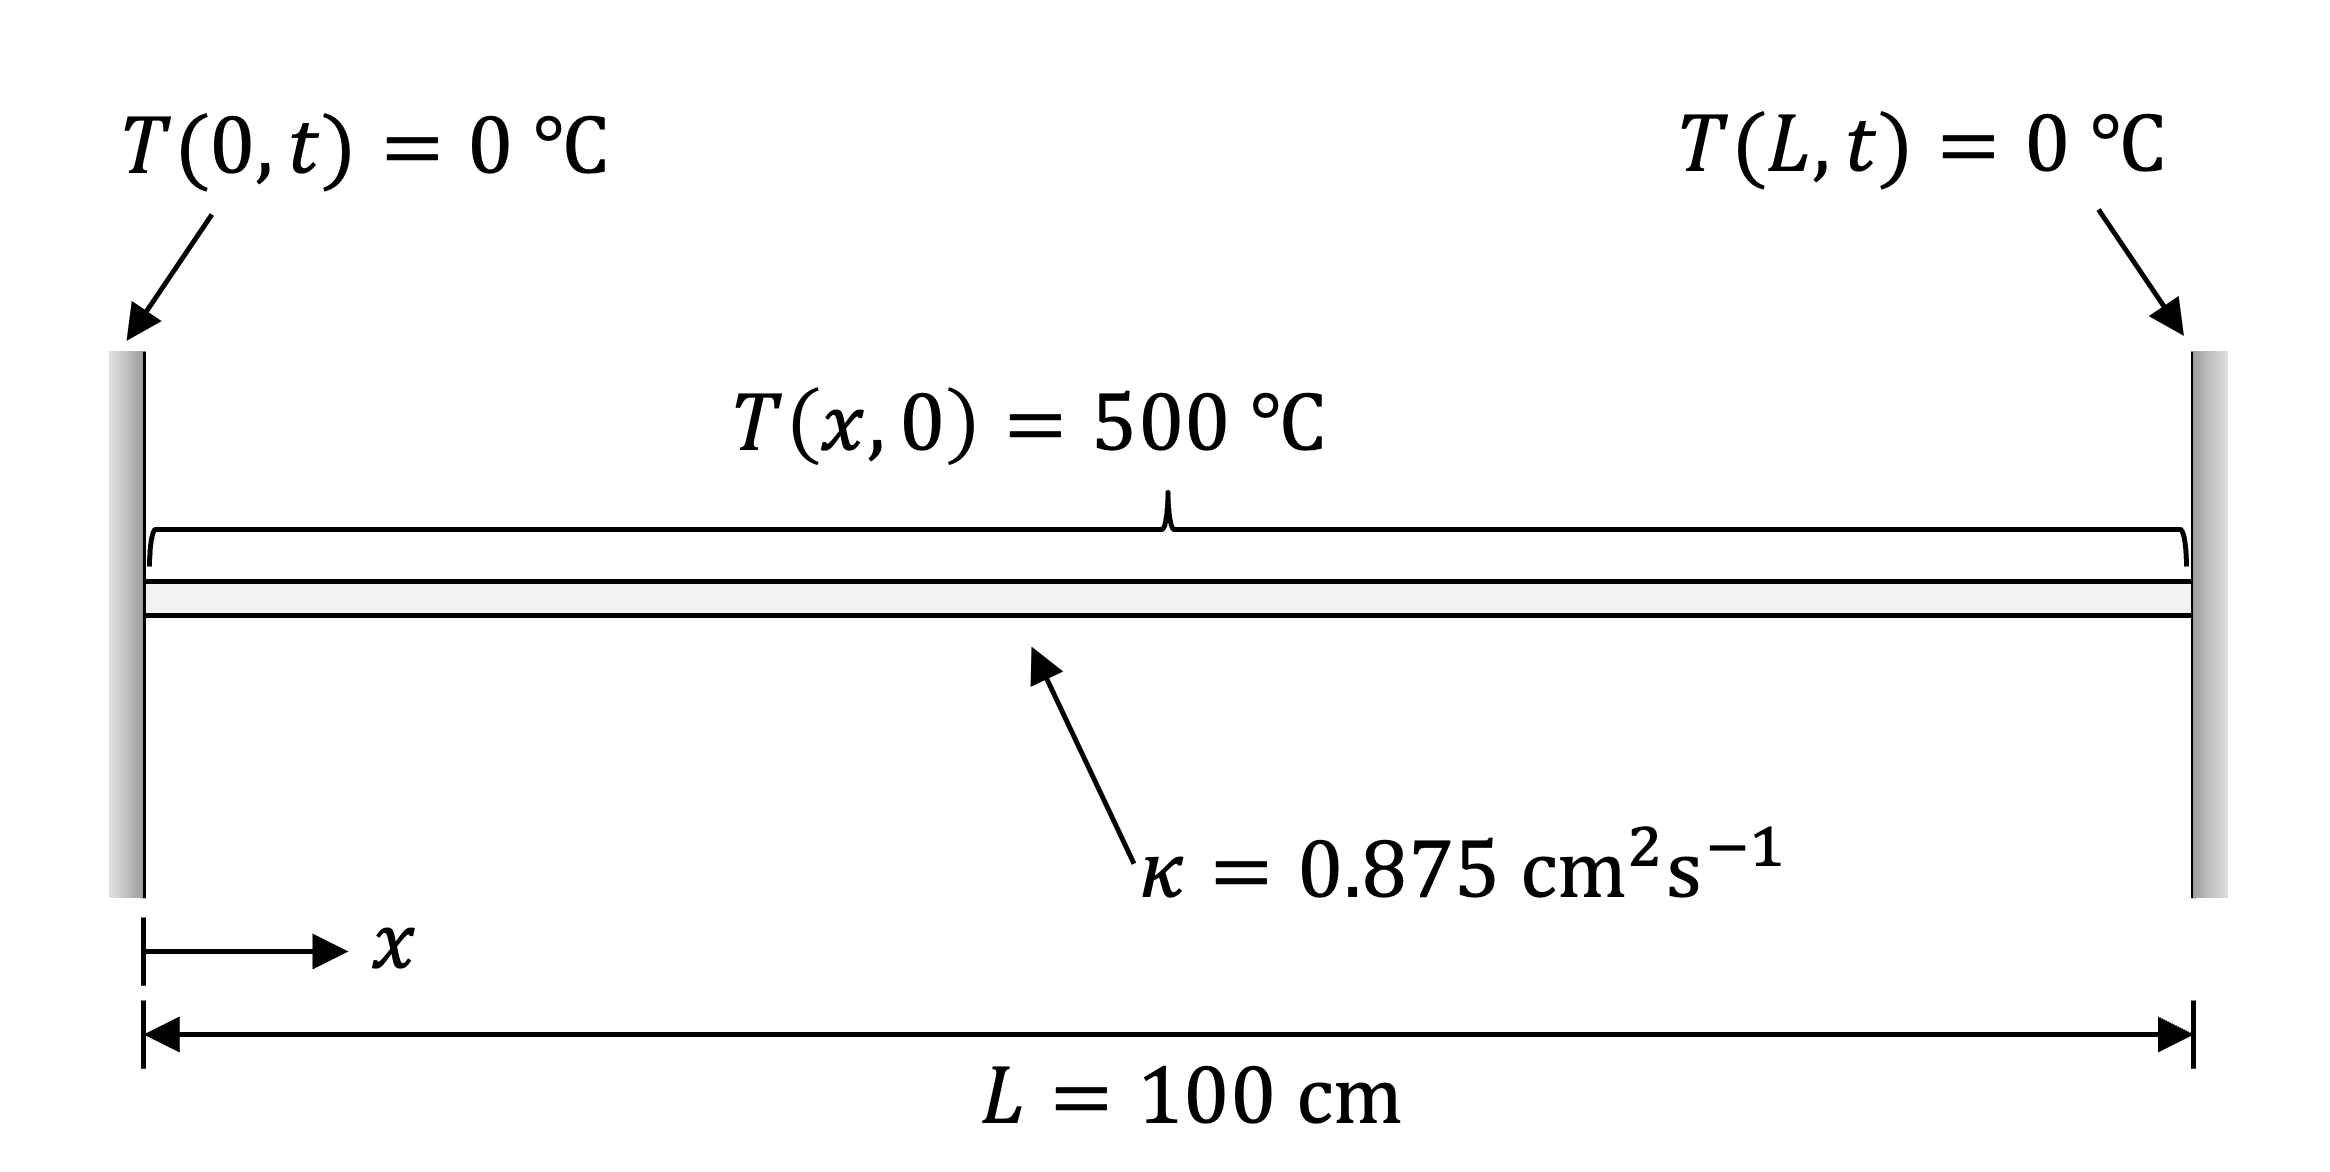
\includegraphics[width=0.9\linewidth]{figs/layout.png}
    \caption{Problem description}
    \label{fig:layout}
\end{figure}

Since we will be using finite difference approximations , it is useful to consider the problem as a two-dimensional grid representing space-time.

\begin{figure}[H]
    \centering
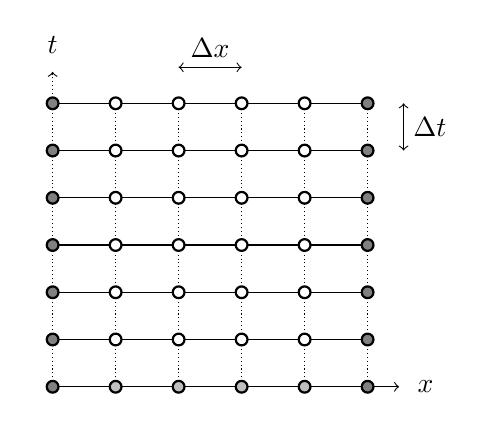
\begin{tikzpicture}
    \matrix (m) [matrix of nodes, nodes in empty cells, nodes={minimum size=0.4cm}, column sep=0.4cm, row sep=0.2cm]{
        &&&&&\\
        &&&&&\\
        &&&&&\\
        &&&&&\\
        &&&&&\\
        &&&&&\\
        &&&&&\\
    };

    \foreach \i in {1,2,3,4,5,6}
        \foreach \j in {2,3,4,5}
            \node[draw, circle, line width=0.8pt, inner sep=1.5pt,] at (m-\i-\j) {};

    \foreach \i in {7}
        \foreach \j in {2,3,4,5}
            \node[fill=lightgray, draw, circle, line width=0.8pt, inner sep=1.5pt,] at (m-\i-\j) {};

    \foreach \i in {1,2,3,4,5,6,7}
        \foreach \j in {1,6}
            \node[fill=gray, draw, circle, line width=0.8pt, inner sep=1.5pt,] at (m-\i-\j) {};

    \foreach \i in {2,3,4,5,6,7}
        \foreach \j in {1, 2,3,4,5,6}
        {
            \pgfmathtruncatemacro{\iprev}{\i-1}
            \draw[densely dotted, shorten <=2pt, shorten >=2pt] (m-\i-\j.center) -- (m-\iprev-\j.center);
        }
    
    \foreach \i in {1,2,3,4,5,6,7}
        \foreach \j in {2,3,4,5,6}
        {
            \pgfmathtruncatemacro{\jprev}{\j-1}
            \draw[shorten <=2pt, shorten >=2pt] (m-\i-\j.center) -- (m-\i-\jprev.center);
        }


    % Drawing the arrows with labels
    \draw[<->] ([yshift=0.25cm]m-1-3.north) -- node[above] {$\Delta x$} ([yshift=0.25cm]m-1-4.north);
    \draw[<->] ([xshift=0.25cm]m-1-6.east) -- node[right] {$\Delta t$} ([xshift=0.25cm]m-2-6.east);
    \draw[->] ([xshift=2pt]m-7-6.center) -- node[xshift=0.5cm] {$x$} ([xshift=0.4cm]m-7-6.center);
    \draw[->, densely dotted] ([yshift=2pt]m-1-1.center) -- node[yshift=0.5cm] {$t$} ([yshift=0.4cm]m-1-1.center);
\end{tikzpicture}
\caption{grid with $\Delta x = 20\ \rm{cm}$ and $\Delta t = 100\ \rm{s}$}
    \label{fig:grid}
\end{figure}

We explore two types of numerical solution to this problem: \textbf{explicit} and \textbf{implicit} solutions.
To evaluate our numerical solutions, the analytical solution is given for Parts I and II is given by {equation \ref{eq:2}}.

\begin{align} \label{eq:2}
    T(x,t) = \frac{2000}{\pi}\sum_{\substack{n=1 \\ n\ \text{odd}}}^{\infty}\frac{1}{n}\sin\frac{n\pi x}{L}e^{-\frac{n^2\pi^2k}{L^2}t}
\end{align}

\subsection{Software setup}
For the software implementation \textbf{Python3} will be used since it has nice linear algebra and calculus tooling (e.g. \textbf{NumPy}, \textbf{SciPy}), and because these tools are very well integrated with \textbf{Matplotlib} which will be use to plot our results.

The code is structured between the \verb|HeatSolver| module and class which solves the heat equation in various ways, and a Notebook to run and visualize the experiments. 
The snippet in figure \ref{code:1} gives some boilerplate for defining the class and implementing the benchmark analytic solution. 

\begin{figure}[H]
\centering
\begin{minted}
[
frame=lines,
baselinestretch=0.8,
fontsize=\scriptsize,
escapeinside=||,
]
{Python3}
@attrs.define
class HeatSolver:
  dx: np.float32
  dt: np.float32
  L: np.float32 = np.float32(100.0)
  k: np.float32 = np.float32(0.875)  
  t_total: np.float32 = np.float32(600.0)
  T_x0: Callable = lambda x: 500.0 * np.ones_like(x)
  T_0t: np.float32 = np.float32(0.0)
  T_Lt: np.float32 = np.float32(0.0)
  
  ...
  
  def _solve_analytic_x_t(self, x , t , N = 100_001):
    x = np.atleast_1d(x)
    t = np.atleast_1d(t)

    ns = np.arange(1, N + 1, 2)
    sums = (1 / ns) * sin(ns[,:] * pi * x[:,] / self.L) @ \
    exp(- ns[:,]**2 * pi**2 * self.k * t[,:] / self.L**2)

    return 2000.0 / np.pi * sums.T
\end{minted}
\captionof{figure}[]{Definition \& Analytic solution code}
\label{code:1}
\end{figure}

The function \verb|_solve_analytic_x_t| takes advantage of Numpy's \textbf{broadcasting} features to compute solutions given vectors $\bm{x_i}$ and $\bm{t_j}$ all in one operation. This optimisation allows using a high precision factor $\bm{N}$ while keeping run-time low. It follows that for any $\Delta x$ and $\Delta t$ we can deduce the vectors defining the discrete grid and sample all the analytical solutions needed.

Within this class we can now define numerical solutions for a general version of the heat equation, and easily compare those solutions against an analytic implementation. 

\end{multicols}

\begin{multicols}{2}
[
\section{Part I: Explicit Solution: Forward Time Centered Space }
]
\subsection{Deriving the update equations}
To derive the FTCS update equations we will use the central difference approximation for the spatial derivative \eqref{eq:3}, and the forward difference approximation for the time derivative \eqref{eq:4}.

\begin{align} 
\frac{\partial^2{T_{i,j}}}{\partial x^2} &= \frac{T_{i+1,j} - 2T_{i,j} + T_{i-1,j}}{\Delta x^2}\label{eq:3} \\
\frac{\partial{T_{i,j}}}{\partial t} &= \frac{T_{i,j+1} - T_{i,j}}{\Delta t}\label{eq:4}
\end{align}

Substituting these into \eqref{eq:1} and rearranging$^{[\rm{\ref{appendix:math1}}]}$ gives the update equation for node $T_{i,j+1}$

\begin{align}\label{eq:5}
T_{i,j+1} &= \lambda T_{i+1,j} + (1 - 2 \lambda)T_{i,j} + \lambda T_{i-1,j} \\
\rm{Where} & \notag \\
\lambda &= \frac{k\Delta t}{\Delta x^2} \notag
\end{align}

This equation gives the following \textbf{computational molecule}.

\begin{figure}[H]
    \centering
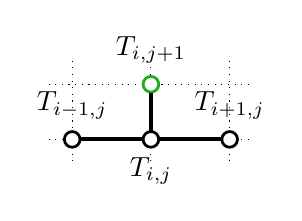
\begin{tikzpicture}
    \matrix (m) [matrix of nodes, nodes in empty cells, nodes={minimum size=0.4cm}, column sep=0.6cm, row sep=0.3cm]{
        &&\\
        &&\\
    };

    \draw[dotted] ([yshift=0.3cm]m-1-1.center) -- ([yshift=-0.3cm]m-2-1.center);
    \draw[dotted] ([yshift=0.3cm]m-1-2.center) -- ([yshift=-0.3cm]m-2-2.center);
    \draw[dotted] ([yshift=0.3cm]m-1-3.center) -- ([yshift=-0.3cm]m-2-3.center);
    \draw[dotted] ([xshift=-0.3cm]m-1-1.center) -- ([xshift=0.3cm]m-1-3.center);
    \draw[dotted] ([xshift=-0.3cm]m-2-1.center) -- ([xshift=0.3cm]m-2-3.center);
    
    \node[fill=white, draw=darkgreen, circle, line width=1pt, inner sep=2pt,] at (m-1-2) {};
    \node[fill=white, draw, circle, line width=1pt, inner sep=2pt,] at (m-2-1) {};
    \node[fill=white, draw, circle, line width=1pt, inner sep=2pt,] at (m-2-2) {};
    \node[fill=white, draw, circle, line width=1pt, inner sep=2pt,] at (m-2-3) {};
    
    \draw[-, line width=1.5pt] ([yshift=-3pt]m-1-2.center) -- ([yshift=3pt]m-2-2.center);
    \draw[-, line width=1.5pt] ([xshift=3pt]m-2-1.center) -- ([xshift=-3pt]m-2-2.center);
    \draw[-, line width=1.5pt] ([xshift=3pt]m-2-2.center) -- ([xshift=-3pt]m-2-3.center);

    \node[above=-2pt of m-1-2] {$T_{i,j+1}$};
    \node[above=-2pt of m-2-1] {$T_{i-1,j}$};
    \node[above=-2pt of m-2-3] {$T_{i+1,j}$};
    \node[below=-3pt of m-2-2] {$T_{i,j}$};
\end{tikzpicture}
\caption{Explicit computational molecule}
    \label{fig:cm}
\end{figure}

Given or boundary conditions and the parabolic nature of the heat equation, we can simply slide the computational molecule left to right bottom to top to compute our approximation.  

\subsection{Software Implementation}

\begin{figure}[H]
\centering
\begin{minted}
[
frame=lines,
baselinestretch=0.8,
fontsize=\scriptsize,
escapeinside=||,
]
{Python3}
def solve_finite_distance(self) -> np.ndarray:
  A = self.k * self.dt / self.dx**2
  B = 1 - 2 * A

  N_x = int(self.L / self.dx + 1)
  N_t = int(self.t_total / self.dt + 1)

  T = np.zeros((N_t, N_x))
  T[0, :] = self.T_x0(np.arange(0, self.L + self.dx, self.dx))
  T[:, 0] = self.T_0t
  T[:, -1] = self.T_Lt

  for j in range(0, N_t - 1):
    for i in range(1, N_x - 1):
        T[j+1, i] = A * (T[j, i+1] + T[j, i-1]) + B * T[j, i]

  return T
\end{minted}
\captionof{figure}[]{Explicit solution}
\label{code:2}
\end{figure}

The algorithm has the consists of the following steps:
\begin{enumerate}[leftmargin=*, itemsep=-2mm, before=\vspace{-7mm}]
    \item Pre-compute the coefficients \verb|A| $= \lambda$ and \verb|B| $= 1 - 2\lambda$
    \item Derive the shape of the solution grid from $\Delta x$, $\Delta t$
    \item Initialize an empty matrix and apply boundaries
\begin{enumerate}[before=\vspace{-3mm}]
    \item Set the row $T_{i,0}$ to $T(\bm{x_i}, 0)$
    \item Set the edge $T_{0,j}$ to $T(0,j)$
    \item Set the edge $T_{L,j}$ to $T(L,j)$
\end{enumerate}
    \item Apply the computational molecule row by row, from the bottom up.
\end{enumerate}
It is important to note that the boundary conditions must be set in that exact order, to maintain the information at the horizontal edges of the rod through time. You might also ask, why does the $t = 0\ \rm{s}$ value take a vector $\bm{x_i}$? This is to prepare for when the function $T(x,0)$ is no longer uniform in Part III. For now, the bottom row is a uniform vector of value $500 ^\circ \rm{C}$.

\subsection{Experiments and analysis}
Three experiments where conducted:
\begin{enumerate}[leftmargin=*, itemsep=-2mm]
    \item  Plotting the temperature distribution over the length of the bar at 100s interval with step sizes $\Delta x = 20\rm{cm}, \Delta t = 100\rm{s}$
    \item  Plotting the temperature distribution and error against the analytical solution overtime with step sizes $\bm{\Delta x} = [20,20,10]\rm{cm},\ $$\bm{\Delta t} = [100, 50, 100]\rm{s}$ at $x=20\rm{cm}$, and recording the values at the final time-step 
    \item Plotting the temperature distribution in space overtime for $\Delta x = 10\rm{cm}, \Delta t = 30\rm{s}$
\end{enumerate}


It can be seen in figure \ref{fig:p1_1} that the explicit numerical solution with that step size gives more accurate results towards the center of the bar, and they get more accurate as time progresses.

\begin{figure}[H]
    % \centernig
    \includesvg[width=1.1\columnwidth]{figs/p1_1.svg}
    \captionsetup{justification=raggedright, margin={10mm,0mm}}
    \caption{$T\ \rm{vs.}\ x,\ \Delta x = 20\rm{cm}, \Delta t = 100\rm{s} $}
    \label{fig:p1_1}
\end{figure}

The same trend can also be confirmed in figure \ref{fig:p1_2} for the first two step size pairs, seeing that the error trends to 0 \textit{asymptotically}. This indicates that for these step size values this method is stable.

Moreover, in the same figure it is apparent that the approximation fails to converge on the solution when the step size is set to $\Delta x = 10\rm{cm}$ and $\Delta t = 100\rm{s}$, it is \textit{unstable}. 

This can be verified theoretically as well. The stability condition for equation \eqref{eq:5} as a solution to the heat equation is given by the following:
\begin{align}
    (1-2\lambda) &\ge 0 \notag \\
    \Longrightarrow \frac{k\Delta t}{\Delta x^2} &\le \frac{1}{2} \label{eq:6}
\end{align}
Substituting $\Delta x$ and $\Delta t$ in equation \eqref{eq:6} gives
\begin{align}
\frac{k\Delta t}{\Delta x^2} = \frac{0.875 \cdot 100}{10^2} &> \frac{1}{2}
\end{align}
which clearly breaks the stability condition. Hence, it can be concluded that the implementation behaves as expected, as this oscillation and increasing magnitude of the error is a feature of the method, not a bug in the implementation \textit{(e.g. precision issue)}. 

\vspace{-3mm} 
\begin{figure}[H]
    \includesvg[width=1.1\columnwidth]{figs/p1_2.svg}
    \captionsetup{justification=raggedright, margin={10mm,0mm}}
        \caption{$T\ \rm{vs.}\ t \text{ at } x = 20\rm{cm}$ explicit}
    \label{fig:p1_2}
\end{figure}

A observation on figure \ref{fig:p1_2} is the fact that, as expected, out of the two stable configurations tested, the one with a finer grid is also the one with the better approximation. This observation enforces the idea that as long as the stability threshold is not crossed lowering either the step-size yields better accuracy.   

\begin{table}[H]
\centering
\small
\begin{tabular}{ |p{1.2cm}||p{1.2cm}|p{1.2cm}|p{1.2cm}|p{1.1cm}| }
 \hline
 \rowcolor{gray!50}
 $\Delta x / \Delta t$ & 20\ /\ 100 & 20\ /\ 50 & 10\ /\ 100 & analytic \\
 \hline 
 $T (^\circ C)$ & 215 & 219 & -3161 & 225 \\
 \hline
 abs. err. & 10 & 6 & 3386 & \\
 \hline
\end{tabular}
\caption{$T (^\circ C)$ and error at $t=600\rm{s}$}
\label{table:1}
\end{table}

Finally, figures \ref{fig:p1_3a}  and \ref{fig:p1_3b} are 3-dimensional visualisations of the Temperature distribution and Absolute Error of the approximations made for step sizes  $\Delta x = 10\rm{cm}$ and $\Delta t = 30\rm{s}$, chosen to be granular, but without becoming unstable. 
 
\begin{figure}[H]
    % \centernig
    \includesvg[width=1.1\columnwidth]{figs/p1_3a.svg}
    \captionsetup{justification=raggedright, margin={10mm,0mm}}
    \caption{$T(x, t)$ with $\Delta x = 10\rm{cm}, \Delta t = 30\rm{s}$}
    \label{fig:p1_3a}
\end{figure}


In figure \ref{fig:p1_3b} it can be seen that the assumption made above regarding the error converging towards 0 overtime holds. The nodes with the largest Absolute Error ($\sim 40 ^\circ C$) occur at one lengthwise extremities at the first time-step ($T_{1,1}, T_{L-1,1}$), this corresponds to the region in the temperature distribution in figure \ref{fig:p1_3a} with the steepest slope; as that slope smooths out overtime, so does the error.

\begin{figure}[H]
    % \centernig
    \includesvg[width=1.1\columnwidth]{figs/p1_3b.svg}
    \captionsetup{justification=raggedright, margin={10mm,0mm}}
    \caption{AE with $\Delta x = 10\rm{cm}, \Delta t = 30\rm{s}$}
    \label{fig:p1_3b}
\end{figure}

Therfore, the conclusion can be drawn that an accurate implementation of the explicit numeric solution has been achieved. It computes better results overtime and towards the center of the bar, but it is unstable for step sizes that break the inequality in \ref{eq:6}.

\end{multicols}

\begin{multicols}{2}
[
\section{Part II: Implicit Solution: Crank-Nicolson Method}
\subsection{Deriving the update equations}
To derive the update equations with the Crank-Nicolson Method, the derivatives at the time midpoint between two time steps are considered, given by the time derivative \eqref{eq:8} and the space derivative \eqref{eq:9}
\begin{align}
\frac{\partial T}{\partial t}\bigg\rvert_{i,j+\frac 1 2} &= \frac{1}{\Delta t} (T_{i,j+1} - T_{i,j}) \label{eq:8}\\
\frac{\partial^2 T}{\partial x^2}\bigg\rvert_{i,j+\frac 1 2} &= \frac{1}{2\Delta x^2}(T_{i-1,j} - 2T_{i,j} + T_{i+1,j} + T_{i-1,j+1} - 2T_{i,j+1} + T_{i+1,j+1}) \label{eq:9}:
\end{align}
Substituting these into \eqref{eq:1} and rearranging$^{[\ref{appendix:math2}]}$ gives the update scheme for the Crank-Nicolson method, in which the left hand side contains unknown values and the right hand side contains known values.
\begin{align}
\lambda T_{i-1,j+1} + \overbrace{(- 2 - 2\lambda)}^{\alpha}T_{i,j+1} + \lambda T_{i+1,j+1} = -\lambda T_{i-1,j} + \overbrace{(2\lambda - 2)}^{\beta} T_{i,j} - \lambda T_{i+1,j} \label{eq:10}
\end{align}
]
This equation gives the computational molecule in figure \ref{fig:cm2}.

We can now construct a system of equations from all the interior nodes at a particular time step to compute all the interior nodes at the next time step. To that end, the following two matrices and bias vector are constructed to encode this system of equations:

\columnbreak

\begin{figure}[H]
    \centering
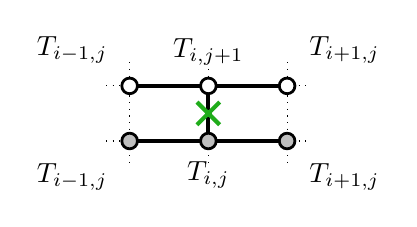
\begin{tikzpicture}
    \matrix (m) [matrix of nodes, nodes in empty cells, nodes={minimum size=0.4cm}, column sep=0.6cm, row sep=0.3cm]{
        &&\\
        &&\\
    };

    \draw[dotted] ([yshift=0.3cm]m-1-1.center) -- ([yshift=-0.3cm]m-2-1.center);
    \draw[dotted] ([yshift=0.3cm]m-1-2.center) -- ([yshift=-0.3cm]m-2-2.center);
    \draw[dotted] ([yshift=0.3cm]m-1-3.center) -- ([yshift=-0.3cm]m-2-3.center);
    \draw[dotted] ([xshift=-0.3cm]m-1-1.center) -- ([xshift=0.3cm]m-1-3.center);
    \draw[dotted] ([xshift=-0.3cm]m-2-1.center) -- ([xshift=0.3cm]m-2-3.center);

    \draw[-, line width=1.5pt] (m-1-1.center) -- (m-1-3.center);
    \draw[-, line width=1.5pt] (m-2-1.center) -- (m-2-3.center);
    \draw[-, line width=1.5pt] (m-1-2.center) -- (m-2-2.center);
    
    \node[fill=white, draw, circle, line width=1pt, inner sep=2pt,] at (m-1-1) {};
    \node[fill=white, draw, circle, line width=1pt, inner sep=2pt,] at (m-1-2) {};
    \node[fill=white, draw, circle, line width=1pt, inner sep=2pt,] at (m-1-3) {};
    \node[fill=lightgray, draw, circle, line width=1pt, inner sep=2pt,] at (m-2-1) {};
    \node[fill=lightgray, draw, circle, line width=1pt, inner sep=2pt,] at (m-2-2) {};
    \node[fill=lightgray, draw, circle, line width=1pt, inner sep=2pt,] at (m-2-3) {};
    \crossnode[draw=darkgreen, line width=1.5pt]{$(m-1-2)!0.5!(m-2-2)$};
    
    \node[above=-2pt of m-1-2] {$T_{i,j+1}$};
    \node[above left=-2pt of m-1-1] {$T_{i-1,j}$};
    \node[above right=-2pt of m-1-3] {$T_{i+1,j}$};
    \node[below left=-2pt of m-2-1] {$T_{i-1,j}$};
    \node[below right=-2pt of m-2-3] {$T_{i+1,j}$};
    \node[below=-2pt of m-2-2] {$T_{i,j}$};
\end{tikzpicture}
\caption{Implicit computational molecule}
    \label{fig:cm2}
\end{figure}

\end{multicols}

\begin{align*}
\overbrace{
\begin{bmatrix}
     \alpha & \lambda & & & & \\
     \lambda & \alpha & \lambda & & & \\ 
     & \lambda & \sddots & \sddots & & \\ 
     & & \sddots & \sddots & \lambda \\
     & & & \lambda & \alpha \\
\end{bmatrix}
}^{A}
\times
\begin{bmatrix}
     T_{1,j+1} \\
     T_{2,j+1} \\
     T_{3,j+1} \\
     \svdots \\
     T_{L-1,j+1} \\
\end{bmatrix}
&=
\overbrace{
\begin{bmatrix}
     \beta & -\lambda & & & & \\
     -\lambda & \beta & -\lambda & & & \\ 
     & -\lambda & \sddots & \sddots & & \\ 
     & & \sddots & \sddots & -\lambda \\
     & & & -\lambda & \beta \\
\end{bmatrix}
}^{B}
\times
\begin{bmatrix}
     T_{1,j} \\
     T_{2,j} \\
     T_{3,j} \\
     \svdots \\
     T_{L-1,j} \\
\end{bmatrix} + 
\overbrace{
\begin{bmatrix}
    -\lambda T_{0,j+1} -\lambda T_{0,j} \\
    \\
    \\
    \\
    -\lambda T_{L,j+1} -\lambda T_{L,j} \\
\end{bmatrix}
}^{\bm b}
\end{align*}
Which can be written in the form 
\begin{align}\label{eq:11}
A \bm{T_{j+1}} &= B \bm{T_{j}} + \bm b\ .
\end{align}
Equation \eqref{eq:11} gives a row-by-row update scheme for the Crank-Nicolson model. To solve this equation for the vector $\bm{T_{j+1}}$ we can use the Thomas Algorithm\supercite{thomas}, since the matrix $A$ is a tridiagonal matrix.

\begin{multicols}{2}
\subsection{Software Implementation}
\begin{figure}[H]
\centering
\begin{minted}
[
frame=lines,
baselinestretch=0.8,
fontsize=\scriptsize,
escapeinside=||,
]
{Python3}
def solve_crank_nicolson(self) -> np.ndarray:
  lmbd = self.k * self.dt / self.dx**2 
  alph, beta = - 2 * lmbd - 2, - 2 * lmbd + 2
  N_x, N_t = int(self.L/self.dx)-1, int(self.t_total/self.dt)+1
  
  Ab = np.zeros((3, N_x))
  Ab[0, 1:] = [lmbd] * (N_x - 1)         
  Ab[1, :] = [alph] * N_x
  Ab[2, :-1] = [lmbd] * (N_x-1)  
  B = diag([beta] * N_x) + diag([-lmbd] * (N_x - 1), k=1) + \
    diag([-lmbd] * (N_x - 1), k=-1)
  b = np.zeros(N_x)
  b[0] = - 2 * lambda *  self.T_0t
  b[-1] = - 2 * lambda *  self.T_Lt
    
  T = np.zeros((N_t, N_x + 2))
  T[0, :] = self.T_x0(self.xs)
  T[:, 0] = self.T_0t
  T[:, -1] = self.T_Lt
  for j in range(N_t - 1):
    T[j+1, 1:-1] = solve_banded((1,1), Ab, B @ T[j, 1:-1] + b)
  return T
\end{minted}
\captionof{figure}[]{Crank Nicolson solution}
\label{code:3}
\end{figure}

\columnbreak
The software implementation differs slightly from equation \eqref{code:3} since it uses the Scipy function \verb|scipy.linalg.solve_banded|\supercite{scipy}, which does a version of the Thomas algorithm for tridiagonal matrices, but it takes as input the banded\supercite{band} form of the matrix. Next, it simply computes the matrix $B$ and the vector $\bm b$, then initialises the temperature distribution matrix with the boundary conditions, same as Part I, and then applies the computational molecule row by row.

\vspace{-1cm}
\subsection{Experiments and analysis}
In this section, the same 3 experiments in Part I are run to compare between the implicit and the explicit methods.

Figure \ref{fig:p2_1} shows the Crank-Nicolson model gives a closer approximation than the explicit method at the outer inner-nodes and it gets considerably closer to the analytical solution overtime. 

\begin{figure}[H]
    \includesvg[width=1.1\columnwidth]{figs/p2_1.svg}
    \captionsetup{justification=raggedright, margin={8mm,0mm}}
    \caption{$T\ \rm{vs.}\ x,\ \Delta x = 20\rm{cm}, \Delta t = 100\rm{s}$ CN}
    \label{fig:p2_1}
\end{figure}

This can also be seen at $x=20\rm{cm}$ in direct comparison with the explicit model in figure \ref{fig:p2_2}. For every step size, the explicit method yields better results then the other model.

Additionally, at $\Delta x = 10\rm{cm}, \Delta t = 100\rm{s}$, the implicit method is stable, and gives the best results among all other steps, particularly at the first time-step. This is a feature of the Crank-Nicolson method, since it is unconditionally stable for linear problems.


% \vspace{-2mm} 
\begin{figure}[H]
    \includesvg[width=1.1\columnwidth]{figs/p2_2.svg}
    \captionsetup{justification=raggedright, margin={10mm,0mm}}
    \caption{$T\ \rm{vs.}\ t \text{ at } x = 20\rm{cm}$}
    \label{fig:p2_2}
\end{figure}

\begin{table}[H]
\centering
\small
\begin{tabular}{ |p{1.2cm}||p{1.2cm}|p{1.2cm}|p{1.2cm}|p{1.1cm}| }
 \hline
 \rowcolor{gray!50}
 $\Delta x / \Delta t$ & 20\ /\ 100 & 20\ /\ 50 & 10\ /\ 100 & analytic \\
 \hline 
 \cellcolor{gray!25} $T (^\circ C)$ & 223.11 & 223.48 & 223.91 & 224.78 \\
 \hline
 \cellcolor{gray!25} abs. err. & 1.66 & 1.30 & 0.86 & \\
 \hline
\end{tabular}
\caption{$T (^\circ C)$ and error at $t=600\rm{s}$ CN}
\label{table:2}
\end{table}

\columnbreak

The Temperature Distribution over time and space doesn't look very different, so instead the Absolute Error and the difference between the errors of the explicit and implicit methods are shown in figures \ref{fig:p2_3b} and \ref{fig:p2_3c}.    

\begin{figure}[H]
    \includesvg[width=1.1\columnwidth]{figs/p2_3b.svg}
    \captionsetup{justification=raggedright, margin={10mm,0mm}}
    \caption{AE at $\Delta x = 10\rm{cm}, \Delta t = 30\rm{s}$ CN}
    \label{fig:p2_3b}
\end{figure}

In figure \ref{fig:p2_3c}, blue essentially represents where the implicit method gives a lower error than the explicit method. The mean and median error and the standard deviation were recorded for both models in table \ref{table:3}.

\begin{figure}[H]
    \includesvg[width=1.2\columnwidth]{figs/p2_3c.svg}
    \captionsetup{justification=raggedright, margin={10mm,0mm}}
    \caption{ED at $\Delta x = 10\rm{cm}, \Delta t = 30\rm{s}$ CN}
    \label{fig:p2_3c}
\end{figure}

\begin{table}[H]
\centering
\small
\begin{tabular}{ |p{1.8cm}||p{1cm}|p{1cm}|p{1cm}| }
 \hline
 \rowcolor{gray!50} model & mean & std & median \\
 \hline
 \cellcolor{gray!25} explicit & 3.73 & 5.77 & 2.99 \\
 \hline 
 \cellcolor{gray!25} implicit (CN) & 1.83 & 2.67 & 0.96 \\
 \hline
\end{tabular}
\caption{mean, median and std comparison}
\label{table:3}
\end{table}
Across the board, the Crank-Nicolson method shows great improvement over the explicit model thanks to the unconditional stability and better overall accuracy. This is due to the method's formulation as a weighted average of the \textit{(explicit)} Forward Time Centered Space and the \textit{(implicit)} Backward Time Centered Space methods, effectively balancing between the stability of the implicit scheme and the accuracy of the explicit scheme.

\end{multicols}

\begin{multicols}{2}
[
\section{Part III: Modelling the Initial Temperature Change}
]
\subsection{Problem setup}
In this section, the bar's  temperature distribution changes \eqref{eq:12}, and we are interested in the first $60\rm{s}$ of cooling.
\begin{align}\label{eq:12}
T(x,0) = -xg(x-L) + c && g = 0.1,\ c = 400  
\end{align}

The challenge comes from the lack of an analytical solution to the new model so there isn't a straightforward way to validate the implementation against. 

\subsection{Software Implementation}
The way boundary conditions are applied in software makes it straightforward to accommodate this change. So far, \verb|HeatSolver.T_x0| has been a function that returns $500$ at all inputs. It then can be replaced with the one in equation \eqref{eq:12}

\begin{figure}[H]
\centering
\begin{minted}
[
frame=lines,
baselinestretch=0.8,
fontsize=\scriptsize,
escapeinside=||,
]
{Python3}
# In the numerical solution method
T[0, :] = self.T_x0(self.xs)
 
          ...

# When using the solver
hs = HeatSolver(dx=dx, dt=dt, t_total=60)
hs.T_x0 = lambda x: -x * g * (g - hs.L) + c
\end{minted}
\captionof{figure}[]{Non-uniform initial state}
\label{code:4}
\end{figure}

This means the the rest of the implementation can remain unchanged.

Additionally, to further analyse and compare numerical solutions , a Backward Time Centered Space solution has also been implemented$^{[\ref{appendix:code1}]}$, which uses a backward difference approximation for the time derivative. This produces$^{[\text{\ref{appendix:math3}}]}$ the update scheme in equation \eqref{eq:13} and the computational molecule in figure \ref{fig:cm3}.
\begin{align}\label{eq:13}
\lambda T_{i+1,j} - (1 + 2\lambda)T_{i,j} + \lambda T_{i+1,j} = - T_{i,j-1} 
\end{align}
\begin{figure}[H]
    \centering
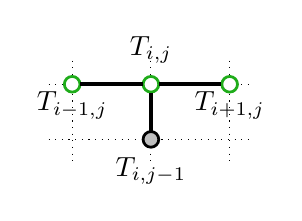
\begin{tikzpicture}
    \matrix (m) [matrix of nodes, nodes in empty cells, nodes={minimum size=0.4cm}, column sep=0.6cm, row sep=0.3cm]{
        &&\\
        &&\\
    };

    \draw[dotted] ([yshift=0.3cm]m-1-1.center) -- ([yshift=-0.3cm]m-2-1.center);
    \draw[dotted] ([yshift=0.3cm]m-1-2.center) -- ([yshift=-0.3cm]m-2-2.center);
    \draw[dotted] ([yshift=0.3cm]m-1-3.center) -- ([yshift=-0.3cm]m-2-3.center);
    \draw[dotted] ([xshift=-0.3cm]m-1-1.center) -- ([xshift=0.3cm]m-1-3.center);
    \draw[dotted] ([xshift=-0.3cm]m-2-1.center) -- ([xshift=0.3cm]m-2-3.center);
    
    \node[fill=white, draw=darkgreen, circle, line width=1pt, inner sep=2pt,] at (m-1-1) {};
    \node[fill=white, draw=darkgreen, circle, line width=1pt, inner sep=2pt,] at (m-1-2) {};
    \node[fill=white, draw=darkgreen, circle, line width=1pt, inner sep=2pt,] at (m-1-3) {};
    \node[fill=lightgray, draw, circle, line width=1pt, inner sep=2pt,] at (m-2-2) {};
    
    \draw[-, line width=1.5pt] ([yshift=-3pt]m-1-2.center) -- ([yshift=3pt]m-2-2.center);
    \draw[-, line width=1.5pt] ([xshift=3pt]m-1-1.center) -- ([xshift=-3pt]m-1-2.center);
    \draw[-, line width=1.5pt] ([xshift=3pt]m-1-2.center) -- ([xshift=-3pt]m-1-3.center);

    \node[above=-2pt of m-1-2] {$T_{i,j}$};
    \node[above=-2pt of m-2-1] {$T_{i-1,j}$};
    \node[above=-2pt of m-2-3] {$T_{i+1,j}$};
    \node[below=-3pt of m-2-2] {$T_{i,j-1}$};
\end{tikzpicture}
\caption{BTCS computational molecule}
    \label{fig:cm3}
\end{figure}

\subsection{Experiments and analysis}
Since there is no analytical solution to benchmark against, 3 different experiments are conducted. Firstly, the solution is approximated with CN at different step-sizes (halving $\Delta x$ and $\Delta t$ at each iteration) and the difference between the results at the current iteration and the result in the previous iteration (i.e. the approximation with double $\Delta x$ and $\Delta t$) is computed. From this data, the difference across time and space is plotted in figure \ref{fig:p3_d}, and the mean and standard deviation of each difference is recorded in table \ref{table:4}.

\vspace{-1cm}
\begin{table}[H]
\centering
\small
\begin{tabular}{ |p{1.2cm}||p{1.2cm}|p{1.2cm}|p{1.2cm}|p{1.35cm}| }
 \hline
 \rowcolor{gray!50}
 $\Delta x / \Delta t$ & 10\ /\ 5 & 5\ /\ 2.5 &  2.5/1.25 & 1.25/0.625 \\
 \hline 
 \cellcolor{gray!25} mean & 4.27 & 2.64 & 0.84 & 0.22 \\
 \hline
 \cellcolor{gray!25} std. & 6.35 & 4.30 & 2.07 & 0.82 \\
 \hline
\end{tabular}
\caption{mean and std. of difference between $2\Delta x$, $2\Delta t$ CN and $\Delta x$, $\Delta t$ CN}
\label{table:4}
\end{table}

The mean over the decreasing step-sizes tends towards 0. This indicates that the approximation is converging on an answer. The standard deviation also tends towards 0; its \textit{larger} values stem from the extremities at the first time steps, where the rate of change of the temperature of the bar is largest, similar to what was observed in parts I and II.

Next, the solutions are approximated at at different step-size resolutions with the CN, FCTS and BTCS models, The CN models' temperature distributions are show in figure \ref{fig:p3_c}, together with the difference between the CN and the FTCS and BTCS distributions.

It can be observed that the surface of the difference tends to flatten out overall as the resolution increases, with the exception of the spatial extremities at the first time-steps where the difference tends to grow. This is in accordance with what was seen in Part II, and can be theoretically justified by the idea that both FTCS and BTCS models fail to capture the regions with more abrupt changes in the temperature distribution.  

However, the fact that, in general, the difference surface tends to flatten out at 0, in both experiments, indicates that the CNN algorithm is converging on an accurate solution.
    
\end{multicols}
\begin{figure}[H]
    \hspace*{-0.5cm}
    \includesvg[width=1\columnwidth]{figs/p3_d.svg}
    \caption{CN Methods difference of previous approximation. Sampled at (a) $\Delta x = 5\rm{cm},$ $\Delta t = 10\rm{s}$, (b) $\Delta x = 2.5\rm{cm}, \Delta t = 5\rm{s}$, (c) $\Delta x = 1.25\rm{cm}, \Delta t = 2.5\rm{s}$, (d) $\Delta x = 0.625\rm{cm}, \Delta t = 1.25\rm{s}$}
    \label{fig:p3_d}
\end{figure}

The reason behind the differences in figure \ref{fig:p3_c} (.2) and (.3) being inverted in sign can be theoretically justified by the idea mentioned in part II, that the CN model is a weighted average of the FCTS and BCTS models. 

\begin{figure}[H]
    \hspace*{-0.5cm}
    \includesvg[width=1.1\columnwidth]{figs/p3_c.svg}
    \caption{(.1) Temperature Distribution (.2) FTCS vs. CN Difference (.3) BTCS vs. CN Difference. Sampled (a) $\Delta x = 20\rm{cm},$ $\Delta t = 10\rm{s}$, (b) $\Delta x = 10\rm{cm}, \Delta t = 5\rm{s}$, (c) $\Delta x = 5\rm{cm}, \Delta t = 2.4\rm{s}$, (d) $\Delta x = 2.5\rm{cm}, \Delta t = 1.2\rm{s}$}
    \label{fig:p3_c}
\end{figure}

When considering computational effort, the implicit FTCS method is the most lightweight, allowing nodes at the same time-step to be computed independently, which opens the door for parallelisation. Both explicit methods, require solving a linear system of equations, which is more computationally intensive than the FTCS scheme. The difference between BTCS and CN is that the latter takes two more terms into account (i.e. $T_{i-1,j}$ and ${T_{i+1,j}}$). This justifies why CN tends to give results with lower temperatures than BTCS: the $0 ^\circ C$ ends of the bar propagate their \textit{coldness} slower overtime, since the BTCS model only takes into account one the \textit{center} node from the previous time-step.

Finally, a \textbf{defect} analysis, inspired by \textit{"Check 3"} in this article\supercite{ver} is performed. The defect is calculated using the numerical approximation of the PDE by subtracting the right-hand side of the equitation from the left-hand side and determine how close to 0 the result is.
\begin{align}
    D(x,t) = \frac{\partial^2 T_{\rm{nm}}(x,t)}{\partial x^2} - \frac{1}{k} \frac{\partial T_{\rm{nm}}(x,t)}{\partial t}  
\end{align}
\par
This defect is calculated at every discrete node using \eqref{eq:3} and \eqref{eq:4} by substituting the numerical solution, giving a metric of the accuracy with which it respects the PDE it was generated from, plotted in figure \ref{fig:p3_e}.

\begin{figure}[H]
    \hspace*{-0.5cm}
    \includesvg[width=1.1\columnwidth]{figs/p3_e.svg}
    \caption{$t$ vs. $x$ vs. Defect. Sampled at (a) $\Delta x = 10\rm{cm},$ $\Delta t = 10\rm{s}$, (b) $\Delta x = 5\rm{cm}, \Delta t = 2.85\rm{s}$, (c) $\Delta x = 2.5\rm{cm}, \Delta t = 0.71\rm{s}$}
    \label{fig:p3_e}
\end{figure}

In order to minimise the defect, $\Delta x$ and $\Delta t$ where chosen such that $\lambda^\eqref{eq:5}$ was less then $0.1$. This works because if $\Delta x$ and $\Delta t$ were to be sampled as they were previously, by being halved, $\lambda$, which has an impact in the accuracy of the model, would change more dramatically, giving a large defect at the two extremities in the first time-step. With the ratio preserved, the results obtained are closer to optimal, with the mean defect and standard deviation are recorded in table \ref{table:5}.

\begin{table}[H]
\centering
\small
\begin{tabular}{ |p{1.2cm}||p{1.2cm}|p{1.2cm}|p{1.2cm}| }
 \hline
 \rowcolor{gray!50}
 $\Delta x / \Delta t$ & 10\ /\ 10 & 5\ /\ 2.85 &  2.5/0.71 \\
 \hline 
 \cellcolor{gray!25} mean & 0.0265 & 0.0255 & 0.0159 \\
 \hline
 \cellcolor{gray!25} std. & 0.106 & 0.177 & 0.249 \\
 \hline
\end{tabular}
\caption{mean and std. of defect for CN model}
\label{table:5}
\end{table}

This final experiment confirms that the solution on which the CN model converges is accurate. The defect is very close to $0$ for all values, except the points with the highest rate of change in the temperature, at the ends of the rod start of the simulation. 
\subsection{Conclusion}

In this section, 3 experiments were conducted: temperature difference between CN models of different sample rates, temperature difference of CN, FTCS and BTCS models, and a defect analysis for the CN. From the results of these experiments, it can be concluded that a robust implementation of the FTCS, CN and BTCS method has been reached. CN gives the most accurate results and FTCS provides an approximation with the least computations per node.


\section{Final remarks}
This report analysed numerical solutions for the heat conductance equation with parabolic boundary conditions. It was proved that the Crank-Nicolson (CN), Forward Time Centered Space (FTCS), and Backward Time Centered Space (BTCS) methods are effective in solving the heat equation. The comparative analysis highlighted CN's superior accuracy due to its implicit nature and average approximation between time steps. FTCS, being explicit and simpler, offers faster computations but with limited stability and accuracy, particularly for larger time steps. BTCS, similar to CN, provides stability, but with slightly less accuracy.

The experiments conducted underscored the importance of selecting an appropriate numerical method based on the specific requirements of the problem at hand. For problems where accuracy is critical and computational resources are available, the CN method is preferred. However, for quick approximations or when resources are limited, FTCS might be a suitable choice. It's also crucial to consider the stability conditions of each method; for example, FTCS requires adherence to the Courant-Friedrichs-Lewy (CFL) condition to ensure stability.

In conclusion, this report has demonstrated the utility and comparative merits of the CN, FTCS, and BTCS methods for solving the heat equation. By leveraging these insights, engineers and scientists can make informed decisions when modeling heat conduction and other diffusion-based phenomena, leading to more accurate and efficient computational solutions.

\newpage

\printbibliography

% \vfill

\begin{appendices}

\section{Calculating the update equations for FTCS}
\label{appendix:math1}
From \eqref{eq:1}, \eqref{eq:3} and \eqref{eq:4} we get
\begin{align*}
\frac{T_{i+1,j} - 2T_{i,j} + T_{i-1,j}}{\Delta x^2} &= \frac{T_{i,j+1} - T_{i,j}}{k\Delta t} &&| \cdot k\Delta t \tag*{(A1)}\\
\overbrace{\frac{k\Delta t}{\Delta x^2}}^{\lambda}(T_{i+1,j} - 2T_{i,j} + T_{i-1,j}) &= T_{i,j+1} - T_{i,j} \tag*{(A2)}\\
\Longrightarrow \lambda T_{i+1,j} - 2 \lambda T_{i,j} + \lambda T_{i-1,j} &= T_{i,j+1} - T_{i,j} &&| -T_{i,j} \tag*{(A3)}\\
T_{i,j+1} &= \lambda T_{i+1,j} + (1 - 2 \lambda)T_{i,j} + \lambda T_{i-1,j} \tag*{\eqref{eq:5}} 
\end{align*}

\section{Calculating the update equations for CN}
\label{appendix:math2}
\begin{align}
\frac{1}{2\Delta x^2}(T_{i-1,j} - 2T_{i,j} + T_{i+1,j} + T_{i-1,j+1} - 2T_{i,j+1} + T_{i+1,j+1}) &= \frac{1}{k\Delta t} (T_{i,j+1} - T_{i,j}) &&|\cdot k\Delta t\tag*{(B1)} \\
\overbrace{\frac{k\Delta t}{2\Delta x^2}}^\lambda(T_{i-1,j} - 2T_{i,j} + T_{i+1,j} + T_{i-1,j+1} - 2T_{i,j+1} + T_{i+1,j+1}) &= T_{i,j+1} - T_{i,j} t\tag*{(B2)} \\
\Longrightarrow \lambda T_{i-1,j+1} + (- 2 - 2\lambda)T_{i,j+1} + \lambda T_{i+1,j+1} &= -\lambda T_{i-1,j} + (2\lambda - 2)T_{i,j} - \lambda T_{i+1,j} \tag*{\eqref{eq:10}}
\end{align}

\section{Calculating the update equations for BTCS}
\label{appendix:math3}

Equation \eqref{eq:bd} gives the backward difference approximation for the time derivative.
\begin{align}
\frac{\partial{T_{i,j}}}{\partial t} &= \frac{T_{i,j} - T_{i,j-1}}{\Delta t}\label{eq:bd}
\end{align}
From \eqref{eq:1}, \eqref{eq:3} and \eqref{eq:bd} we get
\begin{align*}
\frac{T_{i+1,j} - 2T_{i,j} + T_{i-1,j}}{\Delta x^2} &= \frac{T_{i,j} - T_{i,j-1}}{k\Delta t} &&| \cdot k\Delta t \tag*{(C1)}\\
\overbrace{\frac{k\Delta t}{\Delta x^2}}^{\lambda}(T_{i+1,j} - 2T_{i,j} + T_{i-1,j}) &= T_{i,j} - T_{i,j-1} \tag*{(C2)}\\
\Longrightarrow \lambda T_{i+1,j} - 2 \lambda T_{i,j} + \lambda T_{i-1,j} &= T_{i,j} - T_{i,j-1} &&| -T_{i,j} \tag*{(C3)}\\
\lambda T_{i+1,j} - (2 \lambda + 1) T_{i,j} + \lambda T_{i-1,j} &= - T_{i,j-1} && \tag*{\eqref{eq:13}} 
\end{align*}

\section{Coding the BTCS solver for Part III}
\label{appendix:code1}
Unlike the CN solver here, it was chosen to put all the equations (across time-steps) in a single system and solve for all the solutions, this is done for computational efficiency.
The update scheme computed in \eqref{eq:13} gives the following matrix form, where $\alpha= -(2\lambda + 1)$:
\begin{align*}
\overbrace{
\begin{bmatrix}
     \alpha & \lambda & & & & \\
     \lambda & \alpha & \lambda & & & \\ 
     & \lambda & \sddots & \sddots & & \\ 
     & & \sddots & \sddots & \lambda \\
     & & & \lambda & \alpha \\
     1 & & & & & \alpha & \lambda \\
     & 1 & & & & \lambda & \alpha & \lambda \\
     & & 1 & & & & \lambda & \sddots & \sddots \\
     & & & \sddots & & & & \sddots & \sddots & \lambda \\
     & & & & 1 & & & & \lambda & \alpha \\
\end{bmatrix}
}^{A}
\times
\begin{bmatrix}
     T_{1,1} \\
     T_{2,1} \\
     T_{3,1} \\
     \svdots \\
     T_{I-1,1} \\
     T_{1,2} \\
     T_{2,2} \\
     T_{3,2} \\
     \svdots \\
     \svdots \\
     T_{I-1,J-1}\\
\end{bmatrix}
= 
\overbrace{
\begin{bmatrix}
     -T_{1,0} - \lambda T_{0,1}\\
     -T_{2,0} \\
     -T_{3,0} \\
     \svdots \\
     -T_{I-1,0} - \lambda T_{I,1}\\
      -\lambda T_{0,2}\\
      0\\
      0\\
     \svdots \\
     \svdots \\
     -\lambda T_{I,J-1}\\ 
\end{bmatrix}
}^{B} \tag*{(D1)}
\end{align*}
Which can be solved as a equation of the form $A \bm{x} = B$, with the \verb|numpy.linalg.solve|\supercite{np} function. 

\begin{figure}[H]
\centering
\begin{minted}
[
frame=lines,
baselinestretch=0.8,
fontsize=\scriptsize,
escapeinside=||,
]
{Python3}
def solve_backward_distance(self) -> np.ndarray:
  lmbd = self.k * self.dt / (self.dx**2)
  alph = -(2 * lmbd + 1)
  N_x = int(self.L / self.dx) - 1
  N_t = int(self.t_total / self.dt)
  N = N_x*N_t
    
  A = np.diag([alph] * N) + np.diag([1] * (N-N_x), k=-N_x)
  A_T_im1_j = np.tile([lmbd] * (N_x - 1) + [0], N_t)
  A_T_ip1_j = np.tile([0] + [lmbd] * (N_x - 1), N_t)
  A += np.diag(A_T_im1_j[:-1], k=1) + np.diag(A_T_im1_j[:-1], k=-1)
    
  B = np.zeros(N) + (A_T_im1_j - lmbd) * \
    self.T_0t + (A_T_ip1_j - lmbd) * self.T_Lt
  B[:N_x] -= self.T_x0(np.arange(self.dx, self.L, self.dx))
    
  T = np.linalg.solve(A, B).reshape((N_t, N_x))
  T = np.insert(T, 0, self.T_x0(np.arange(self.dx, self.L, self.dx)), axis=0)
  T = np.insert(T, 0, self.T_0t, axis=1)
  T = np.insert(T, N_x + 1, self.T_Lt, axis=1)
    
  return T
\end{minted}
\captionof{figure}[]{BTCS solver}
\label{code:5}
\end{figure}

\section{Source Archive}
The figures used, along with the Jupyter Notebook, Python script and the TeX source file of this report are hosted on GitHub, at \url{https://github.com/NemoInfo/Mathatical-Systems/tree/main/cw2}

\end{appendices}


\end{document}
